\chapter{Modelos implementados}
\label{chapter:modelos}

En este capítulo vamos a repasar qué modelos he implementado y cómo funcionan cada uno de ellos. Primero se hará una revisión teórica de los modelos y posteriormente un análisis breve del código explicando las particularidades de las implementaciones.

\section{Algoritmos de ensamblaje}

Los algoritmos que he implementado pertenecen a una familia concreta de algoritmos de detección de anomalías denominados como algoritmos de ensamblaje o ``Ensemble Algorithms'' en inglés. Estos algoritmos son lo equivalente a los meta-algoritmos pero destinados a la detección de anomalías. Para dar una mejor definición de qué son los algoritmos de ensamblaje vamos a introducir una clasificación de los mismos para dar las categorías que entran dentro de esta definición.

\begin{itemize}
	\item Algoritmos de ensamblaje secuenciales: En este tipo de algoritmos tenemos un algoritmos base o un conjunto de algoritmos base que se aplican de forma secuencial, de forma que las primeras ejecuciones se ven usadas o modificadas por ejecuciones futuras de algoritmos. Finalmente el resultado puede ser una combinación ponderada de las valoraciones de los algoritmos o el resultado del último de ellos.
	
	
	\begin{algorithm}[H]{\textbf{Ensamblaje secuencial:}}
		\SetAlgoLined
		
		\textbf{Entrada: } Conjunto de datos $\mathcal{D}$, Algoritmos base $\mathcal{A}_1 , ... , \mathcal{A}_r$
		
		j=1
		
		\Repeat{fin}{
			Tomamos el algoritmo $\mathcal{A}_j$ según los resultados anteriores
			
			Tomamos el conjunto de datos modificado $f_j (\mathcal{D})$ de anteriores ejecuciones
			
			Ejecutamos el algoritmo $\mathcal{A}_j$ sobre $f_j (\mathcal{D})$
			
			j=j+1
			
		}
	
		\KwResult{Combinación de los resultados}
	\end{algorithm}
	\item Algoritmos de ensamblaje independientes: En este caso se emplean o bien diferentes instancias del mismo algoritmo o bien diferentes porciones de los datos que se emplearán de forma distinta. Se puede variar la instanciación por ejemplo dependiendo del subespacio sobre el que queramos ejecutarlo o dependiendo de las características de una porción concreta de los datos.
	
	\begin{algorithm}[H]{\textbf{Ensamblaje independiente:}}
		\SetAlgoLined
		
		\textbf{Entrada: } Conjunto de datos $\mathcal{D}$, Algoritmos base $\mathcal{A}_1 , ... , \mathcal{A}_r$
		
		j=1
		
		\Repeat{fin}{
			Tomamos el algoritmo $\mathcal{A}_j$
			
			Creamos el conjunto de datos modificado $f_j (\mathcal{D})$
			
			Ejecutamos el algoritmo $\mathcal{A}_j$ sobre $f_j (\mathcal{D})$
			
			j=j+1
			
		}
		
		\KwResult{Combinación de los resultados}
	\end{algorithm}
\end{itemize}

\section{Mahalanobis Kernel}

Este algoritmo está englobado dentro de la categoría de algoritmos basados en dependencia. Esta clase de algoritmos intenta estudiar las dependencias que existen entre atributos para así poder detectar las instancias u objetos que no tienen estas dependencias y marcarlos como anomalías.

Si intentamos visualizar esta dependencia entre atributos de forma gráfica lo que observaríamos es que los datos están alineados o posicionados en hiperplanos lineales o no lineales de la siguiente forma:

\begin{figure}[H]
	\centering
	\label{hiperplano}
	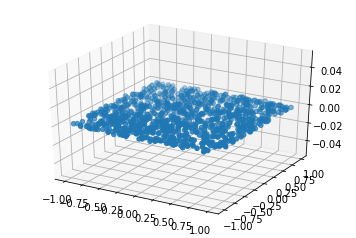
\includegraphics[scale=0.8]{imagenes/hiperplano}
	\caption{Hiperplano}
\end{figure}

Esta figura es un ejemplo clásico de estudio de algoritmos como por ejemplo PCA (algoritmo que quedaría dentro de esta categoría).

\begin{figure}[H]
	\centering
	\label{hiperboloide}
	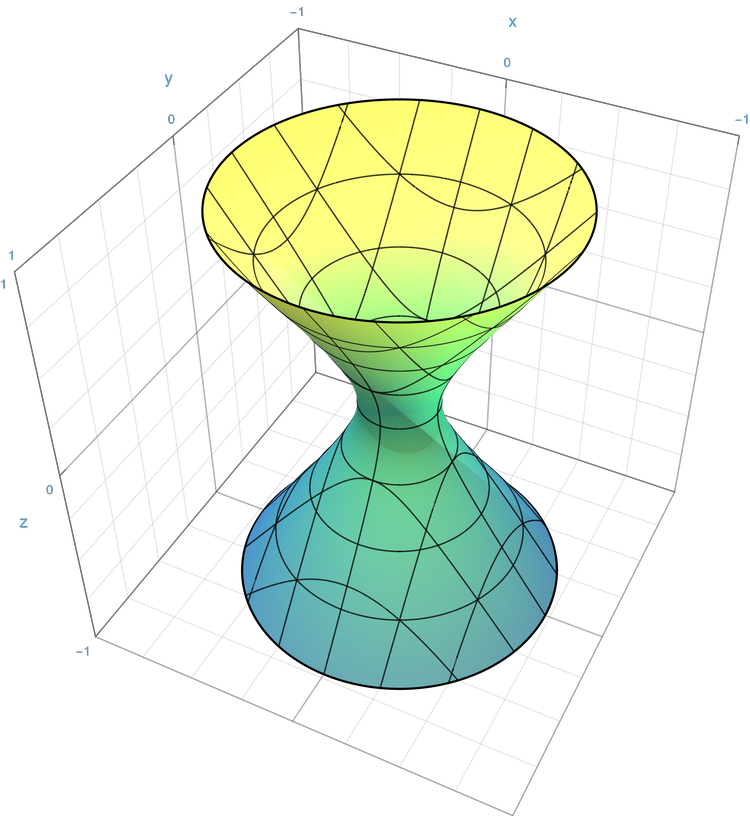
\includegraphics[scale=2.5]{imagenes/hiperboloide}
	\caption{Hiperboloide \href{https://commons.wikimedia.org/wiki/File:Circular_Hyperboloid_Of_One_Sheet_Quadric.png}{Wikimedia}}
\end{figure}

En este caso tenemos el ejemplo de un hiperboloide que no tiene una dependencia lineal, si no que presenta una dependencia de tipo cuadrático.

El método de Mahalanobis Kernel puede ser visto como una modificación de PCA. PCA básicamente dispone de dos pasos:

\begin{enumerate}
	\item Determinar un sistema ortogonal de direcciones principales y proyectar los datos sobre este sistema.
	\item Calcular la distancia entre el punto original y la proyección como su puntuación de anomalía.
\end{enumerate}

El método Mahalanobis Kernel intenta tener este mismo comportamiento en dos pasos y que ahora veremos. El algoritmo PCA es muy útil cuando los datos tienen atributos relacionados en un hiperplano, mientras que Mahalanobis Kernel funciona mejor cuando los datos están relacionados en formas más complejas como el hiperboloide que hemos enseñado. La elección de este algoritmo en vez de PCA recae en el hecho de que PCA es un algoritmo clásico y el escenario en el que mejor funciona (hiperplano) es más restrictivo que el que nos ofrece Mahalanobis Kernel con un abanico de figuras más amplio.

Vamos a describir el funcionamiento del algoritmo, pero primero vamos a introducir notación. Vamos a llamar $D$ a la matriz de datos que está centrada en la media y que tiene dimensiones $n\times d$, es decir, tenemos $n$ instancias u objetos de dimensionalidad $d$.

\begin{algorithm}{\textbf{Mahalanobis Kernel}}
	\caption{Mahalanobis Kernel}
	\label{mahalanobis_kernel}
	\KwIn{$D$}
	
	$S = DD^T$.
	
	$S = Q\Delta^2 Q^T$.
	
	Almacenamos los vectores propios columna no negativos de $Q\Delta$ en una matriz $D'$
	
	Normalizamos $D'$ para que tenga media $0$ y varianza $1$.
	
	$vector\_media = media(D')$
	
	$puntuaciones = []$
	
	\ForEach{fila en D'}{
		$score = distancia(vector\_media , fila)$
		
		$puntuaciones = [puntuaciones, score]$
	}
	\KwOut{puntuaciones}
\end{algorithm}

El algoritmo comienza con la matriz de datos $D$. Se obtiene la matriz simétrica $S$ y se hace la descomposición en valores singulares. 

Con este modelo tenemos las dos fases que teníamos en PCA. Primero obtenemos una matriz $D'$ de los datos proyectados y transformados para posteriormente reportar la puntuación de anomalía como una distancia.

Veamos ahora la implementación en Python.

\begin{lstlisting}[language=Python]
def runMethod(self):
'''
@brief Function that executes the Kernel Mahalanobis method. The results are
stored on the variable self.scores
@param self
'''
''' Compute the S matrix of the algorithm'''
S = np.dot(self.dataset, self.dataset.T)
''' Now we diagonalize it'''
Q,delta_sq,Qt = np.linalg.svd(S)
del S
del Qt
''' Obtain delta as matrix'''
delta = np.matrix(np.diag(np.sqrt(delta_sq)))
del delta_sq
Q = np.matrix(Q)
''' Compute de D' matrix and normalize it'''
Dprime = np.dot(Q,delta)
del Q
del delta
Dp_std = scale(Dprime, axis=1)
del Dprime
''' We compute its mean on the rows to compute the deviation as the score'''
mean = Dp_std.mean(axis=0)
self.outlier_score=[]
''' The score is the euclidean distance to the mean'''
for i in range(len(Dp_std)):
self.outlier_score.append(np.linalg.norm(mean-Dp_std[i])**2)
self.outlier_score = np.array(self.outlier_score)
self.calculations_done=True
\end{lstlisting}

La implementación del algoritmo se ha realizado en Python como el resto del proyecto y posteriormente se explicará en detalle cómo se ha organizado.

El algoritmo basa su implementación en la librería NumPy.